% !TEX root = 0_main.tex
\subsection*{Teilaufgabe 1}
\begin{aufgabe}%1
\begin{teile}
	\item 
	\item 
	\item 
	\item 
	\item 
	\item
	\item 
	\item 
	\item
\end{teile}
\end{aufgabe}

\begin{aufgabe}%2

\end{aufgabe}

\begin{aufgabe}%3

\end{aufgabe}

\begin{aufgabe}%4

  \begin{teile}
  	\item 		 $\{\text{s.vorname} | s \in \text{ Student} \land \forall v \in \text{Vorlesung}(\text{v.Name = 'Datenbanksysteme I'} \Rightarrow \exists b \in \text{besucht}(\text{v.VNR = b.VNR} \land \text{s.MatrikelNr = b. MatrikelNr}))    \}$

  	oder\\
  	$\{s.vorname | s \in Student \land s.MatrikelNr = b.Student \land b \in besucht \land b.vorlesung = v.VNR \land v \in Vorlesung \land v.titel = 'Datenbanksysteme I' \}$

  	\item $\{ \text{s.MatrikelNr} | s \in \text{Student} \land \forall b \in \text{besucht} \Rightarrow \forall v \in Vorlesung (b.Vorlesung = v.VNR \land b.Student = s.Matrikelnummer \Rightarrow v.Klausurtermin \leq 31.12.17 ) \}$ \\
  	oder \\
  	$\{s.Matrikelnummer | s \in Student \land s.MatrikelNr = b.Student \land b \in besucht \land b.Vorlesung = v.VNR \land v \in Vorlesung \land \not\exists (v.Klausurtermin > 31.12.2017) \}$


  \item $\{ s.m | s \in Student \land d.Nachname = Schulz \land d.titel = ProfDr \land d \in Dozent \land \forall v \in Vorlesungen (v.Dozent = d.DNR \Rightarrow \exists b \in besucht (b.Student = s.MatrikelNr \land b.Vorlesung = v.VNR))\}$

  \end{teile}

\end{aufgabe}

\begin{aufgabe}%5
\begin{teile}
	\item 
	\item 
	\item 
\end{teile}
\end{aufgabe}

\begin{aufgabe}%6
	\begin{teile}
		\item 
		\item 
	\end{teile}
\end{aufgabe}

\clearpage

\subsection*{Teilaufgabe 2}
\setcounter{aufgcount}{0}

\begin{aufgabe}%1
  \begin{teile}
    \item
    \begin{itemize}
      \item Die Klasse F implementiert das Interface (die Schnittstelle) I. Sie hat somit alle Funktionalitäten, die als Schnittstelle von der Klasse I zur Verfügung gestellt werden.
      \item Die Klasse X erbt von der abstrakten Oberklasse R.
    \end{itemize}
    \item \mbox{}\\ 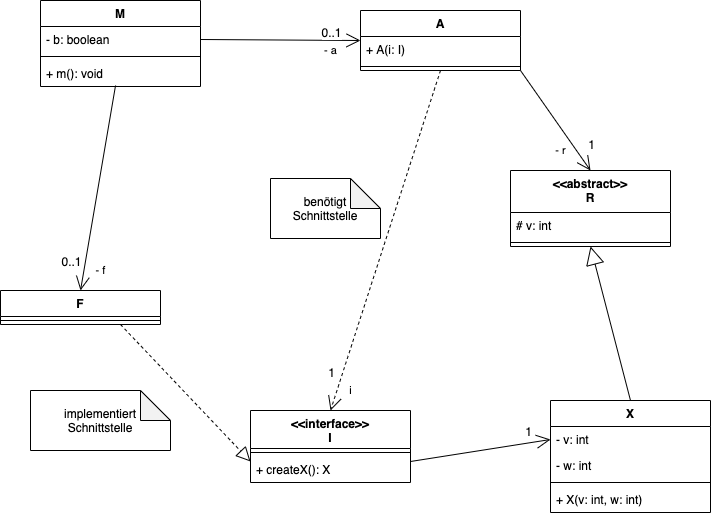
\includegraphics[width = 0.9\linewidth]{F18_66116_T2_TA2_A1b.png}
    \item \mbox{}\\ 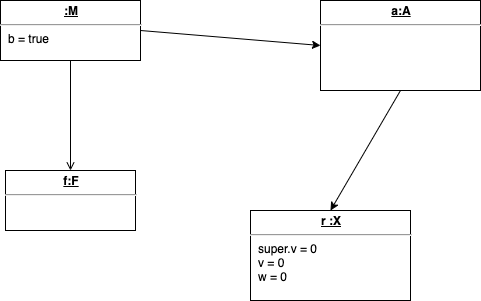
\includegraphics[width = 0.7\linewidth]{F18_66116_T2_TA2_A1c.png}
    \item \mbox{}\\ 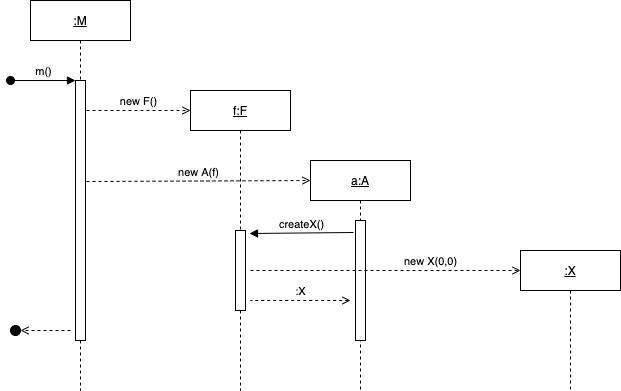
\includegraphics[width = \linewidth]{F18_66116_T2_TA2_A1d.png}
  \end{teile}
\end{aufgabe}

\begin{aufgabe}%2
\begin{teile}
	\item 
	\item 
	\item 
	\item
\end{teile}
\end{aufgabe}

\begin{aufgabe}%3

\end{aufgabe}

\begin{aufgabe}%4
	
\end{aufgabe}
